% Options for packages loaded elsewhere
\PassOptionsToPackage{unicode}{hyperref}
\PassOptionsToPackage{hyphens}{url}
%
\documentclass[
]{article}
\usepackage{amsmath,amssymb}
\usepackage{lmodern}
\usepackage{iftex}
\ifPDFTeX
  \usepackage[T1]{fontenc}
  \usepackage[utf8]{inputenc}
  \usepackage{textcomp} % provide euro and other symbols
\else % if luatex or xetex
  \usepackage{unicode-math}
  \defaultfontfeatures{Scale=MatchLowercase}
  \defaultfontfeatures[\rmfamily]{Ligatures=TeX,Scale=1}
\fi
% Use upquote if available, for straight quotes in verbatim environments
\IfFileExists{upquote.sty}{\usepackage{upquote}}{}
\IfFileExists{microtype.sty}{% use microtype if available
  \usepackage[]{microtype}
  \UseMicrotypeSet[protrusion]{basicmath} % disable protrusion for tt fonts
}{}
\makeatletter
\@ifundefined{KOMAClassName}{% if non-KOMA class
  \IfFileExists{parskip.sty}{%
    \usepackage{parskip}
  }{% else
    \setlength{\parindent}{0pt}
    \setlength{\parskip}{6pt plus 2pt minus 1pt}}
}{% if KOMA class
  \KOMAoptions{parskip=half}}
\makeatother
\usepackage{xcolor}
\IfFileExists{xurl.sty}{\usepackage{xurl}}{} % add URL line breaks if available
\IfFileExists{bookmark.sty}{\usepackage{bookmark}}{\usepackage{hyperref}}
\hypersetup{
  pdftitle={Community Priorities},
  pdfauthor={Jacob Ford, Solstice Data Scientist},
  hidelinks,
  pdfcreator={LaTeX via pandoc}}
\urlstyle{same} % disable monospaced font for URLs
\usepackage[margin=1in]{geometry}
\usepackage{graphicx}
\makeatletter
\def\maxwidth{\ifdim\Gin@nat@width>\linewidth\linewidth\else\Gin@nat@width\fi}
\def\maxheight{\ifdim\Gin@nat@height>\textheight\textheight\else\Gin@nat@height\fi}
\makeatother
% Scale images if necessary, so that they will not overflow the page
% margins by default, and it is still possible to overwrite the defaults
% using explicit options in \includegraphics[width, height, ...]{}
\setkeys{Gin}{width=\maxwidth,height=\maxheight,keepaspectratio}
% Set default figure placement to htbp
\makeatletter
\def\fps@figure{htbp}
\makeatother
\setlength{\emergencystretch}{3em} % prevent overfull lines
\providecommand{\tightlist}{%
  \setlength{\itemsep}{0pt}\setlength{\parskip}{0pt}}
\setcounter{secnumdepth}{-\maxdimen} % remove section numbering
\usepackage{booktabs}
\usepackage{longtable}
\usepackage{array}
\usepackage{multirow}
\usepackage{wrapfig}
\usepackage{float}
\usepackage{colortbl}
\usepackage{pdflscape}
\usepackage{tabu}
\usepackage{threeparttable}
\usepackage{threeparttablex}
\usepackage[normalem]{ulem}
\usepackage{makecell}
\usepackage{xcolor}
\ifLuaTeX
  \usepackage{selnolig}  % disable illegal ligatures
\fi

\title{Community Priorities}
\author{Jacob Ford, Solstice Data Scientist}
\date{2022-08-16}

\begin{document}
\maketitle

\hypertarget{introduction}{%
\section{Introduction}\label{introduction}}

Solar power is the fastest
\href{https://www.c2es.org/content/renewable-energy/\#:~:text=Renewables\%20made\%20up\%20nearly\%2020,the\%20fastest\%2Dgrowing\%20electricity\%20source.}{growing}
renewable energy source. Community shared solar (CSS) projects lower the
barrier to entry. This is accomplished by increasing the applicant pool
by allowing those without rooftop access, such as renters or those in
apartment buildings, and by lowering the financial burden of entry, as
the fixed costs to install and operate the solar panels are
collectivised rather than focused on one rooftop. CSS programs that are
third-party owned and have participants subscribe to ongoing payments.
Typically, within these programs, customers are given predefined,
discrete contract terms rather than being able to compare multiple
offerings or select their own terms. Our research is attempting to mimic
this approach by giving customers a randomly assigned contract and
surveying them on their willingness to adopt this program.

For potential customers, community solar contracts vary by their
contract attributes. These include term length, cancellation fees, and
potential savings rates relative to traditional utility bill companies.
Given the importance of both the solar industry and the relatively
incipient community solar industry, a dearth of research exists on how
potential customer priorities are reflected in the likelihood of
contract adoption.

This research seeks to fill this gap by developing quantitative
measurements of community priorities in likelihood of contract adoption.
An original data set comprised of potential community solar customers
surveyed was collected. Along with respondents demographic information,
draft contracts with varying degrees of contract attributes were shown
to each participant and their contract adoption rates. Using a weighted
logit model, the likelihood of contract adoption was analyzed by
including predictors for various demographic data and contract
attributes. Additionally, relative importance is through a multinomial
logit model, allowing contract attributes and demographic information to
be interpreted in predictive strength relative to respective reference
groups.

\hypertarget{literature-review}{%
\subsection{Literature Review}\label{literature-review}}

\textbf{to-do: to be added/folded into the Introduction to frame the
macro-scope of this study}

\hypertarget{methods}{%
\section{Methods}\label{methods}}

The community solar priorities research consists of an analysis of
survey data in which each respondent was asked to evaluate two
hypothetical community solar contracts with varying contract terms.
Respondents also answered a number of demographic questions.

The contracts that respondents reviewed varied along the following
features: (1) the program's savings rate compared to the typical monthly
electricity bill, (2) the program's cancellation fee, (3) the contract
term's length in years, and (4) the page length of the contract.

In addition to basic descriptive analyses, the goal is to conduct two
distinct analyses using the survey data. The primary analysis will use a
logit model to estimate respondents' stated willingness to enroll in the
contracts they reviewed, controlling for available demographic
characteristics. The secondary analysis will use an order multinomial
logit model to estimate respondents' stated willingness to enroll in a
contract based on various contract terms as measured by a 5-point Likert
scale.

\hypertarget{data-collection}{%
\subsection{Data Collection}\label{data-collection}}

Survey respondents were drawn from two sources: (1) members of the
Qualtrics panel (``the Qualtrics sample''), and (2) individuals in
community groups identified by Solstice (``the Community Group
sample''). Combined, these two surveys represent the primary data
source. Survey responses were collected in the Qualtrics sample from
April 2021 to June 2021, and resulted in 1,261 individual responses. To
expand the survey population, the Community Group sample was collected
from December 2021 to June 2022, with 1,022 responses. Total responses
resulted in 2,283. Response quality was measured in order to detect
fraud or errant submissions. After this prophylactic step, a total of
1,493 unique individuals remained, with a total of 2,986 responses as
each individual reviewed two contracts.

To make sure that enough of the respondents are from populations of
interest, both of these data sources oversampled low-income respondents
and people of color. To avoid biased estimates as a result of the
overweighting in the survey design, survey weights are devised using
state level ACS data for race. Weights are available as well for income,
however due to the dynamic surveying of income used in the design of the
survey weighting was opted for just race controls. Please reference the
\href{https://jake-ford.github.io/SETO_Data_Analysis/survey_weights.html}{survey
weights} section for additional information.

The population for this component of our research is adults (18+) in the
eight states we will include within this study: Massachusetts, New York,
California, Oregon, Illinois, Maryland, Colorado and Minnesota. We have
chosen to oversample-populations that are considered low- to
moderate-income (LMI) defined as up to 50\% and between 50\%-80\% of an
area's median income, in accordance with the Department of Housing and
Urban Development's (HUD) definitions of each
\href{https://www.hudexchange.info/programs/acs-low-mod-summary-data/}{term.}.
Dynamic surveying was deployed in which respondents are asked whether
their income falls within the LMI ranges that correspond with their zip
code and household size. This is the preferred approach for this
research as it allows for comparing priorities across broad income
categories and avoid non- response issues attached to asking respondents
to self-attest their income levels. We have also chosen to oversample
minority and renter populations in this research, surpassing the
proportional estimates of these demographics supplied by the 2020
American Community Survey (ACS) estimates. We have designed this
sampling scheme to center familiarity with community solar as a core
demographic within this research, though we will not weight on this
demographic due to lack of an applicable metric. By centering
familiarity with community solar as a central demographic within this
research, Solstice plans to incorporate respondents that are the likely
next adopters of community solar and respondents from populations that
are not currently effectively reached by community solar. All
demographic information will be self-attested through the community
solar priorities research survey.

Full copies of the survey questions are available on the
\href{https://github.com/Jake-Ford/SETO_Data_Analysis/tree/main/Qualtrics\%20Survey}{github
repository}.

\hypertarget{descriptive-statistics}{%
\subsubsection{Descriptive Statistics}\label{descriptive-statistics}}

Table 1 shows the summary statistics for both the demographic and the
contract attribute data. Contract varying terms such as savings rate,
cancellation fee, contract pages and contract years were evenly divided
so as to evaluate contract adoption rate relative to contract
differences. Contracts were randomly assigned to responsees to review.
The statistics below show how in aggregate, the distribution of contract
attributes remained similar to their construction.

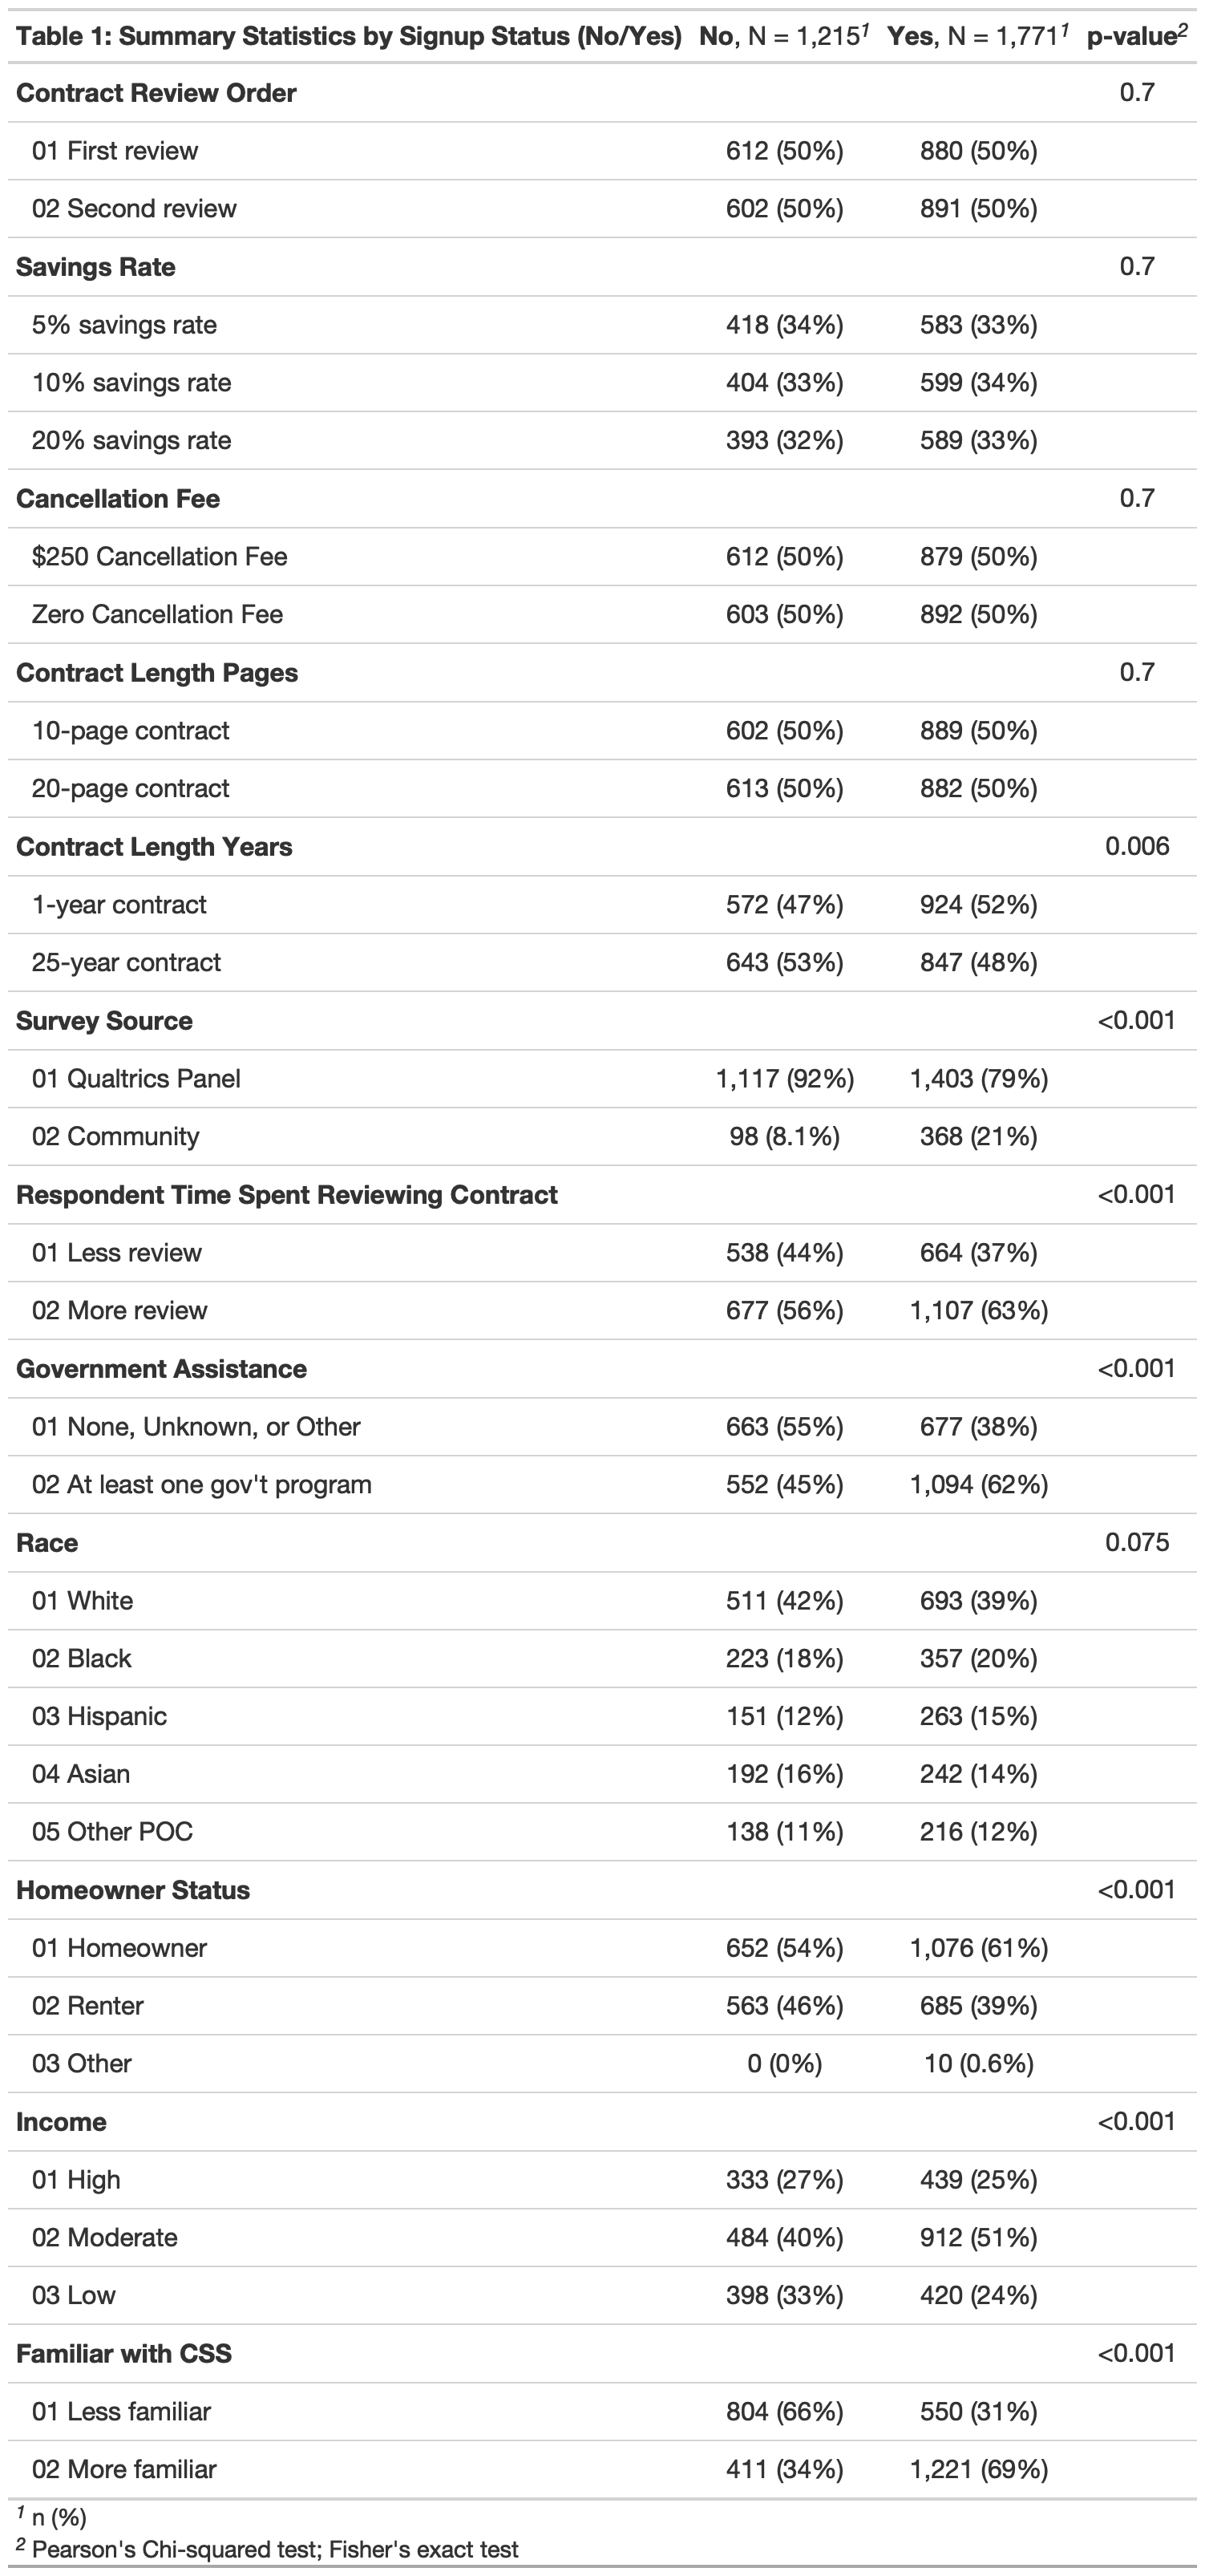
\includegraphics{/Users/jacobford/Documents/GitHub/SETO_Data_Analysis/community_priorities_files/figure-latex/unnamed-chunk-5-1.png}

\hypertarget{demographic-comparison}{%
\subsection{Demographic Comparison}\label{demographic-comparison}}

Demographic data as reported in Table 1 reflects the oversampling of
LMI, minority and renting communities. Graphs 1-3 show the proportion of
each of these oversampled demographic categories in comparison totals.
For race and income, comparison data is taken for the 8 state region
from the 2020 5-year American Community Survey. Given the dynamic
sampling used for income categories, control totals for income is taken
from the Department of Housing and Urban Development's Office of Policy
Development and Research (PD\&R) Comprehensive Housing Affordability
Strategy Data (CHAS). The most recent CHAS data is available as of
\href{https://www.huduser.gov/portal/datasets/cp.html}{2018 5-year
data}.

\hypertarget{race}{%
\subsubsection{Race}\label{race}}

\includegraphics{/Users/jacobford/Documents/GitHub/SETO_Data_Analysis/community_priorities_files/figure-latex/unnamed-chunk-7-1.pdf}

\hypertarget{income}{%
\subsubsection{Income}\label{income}}

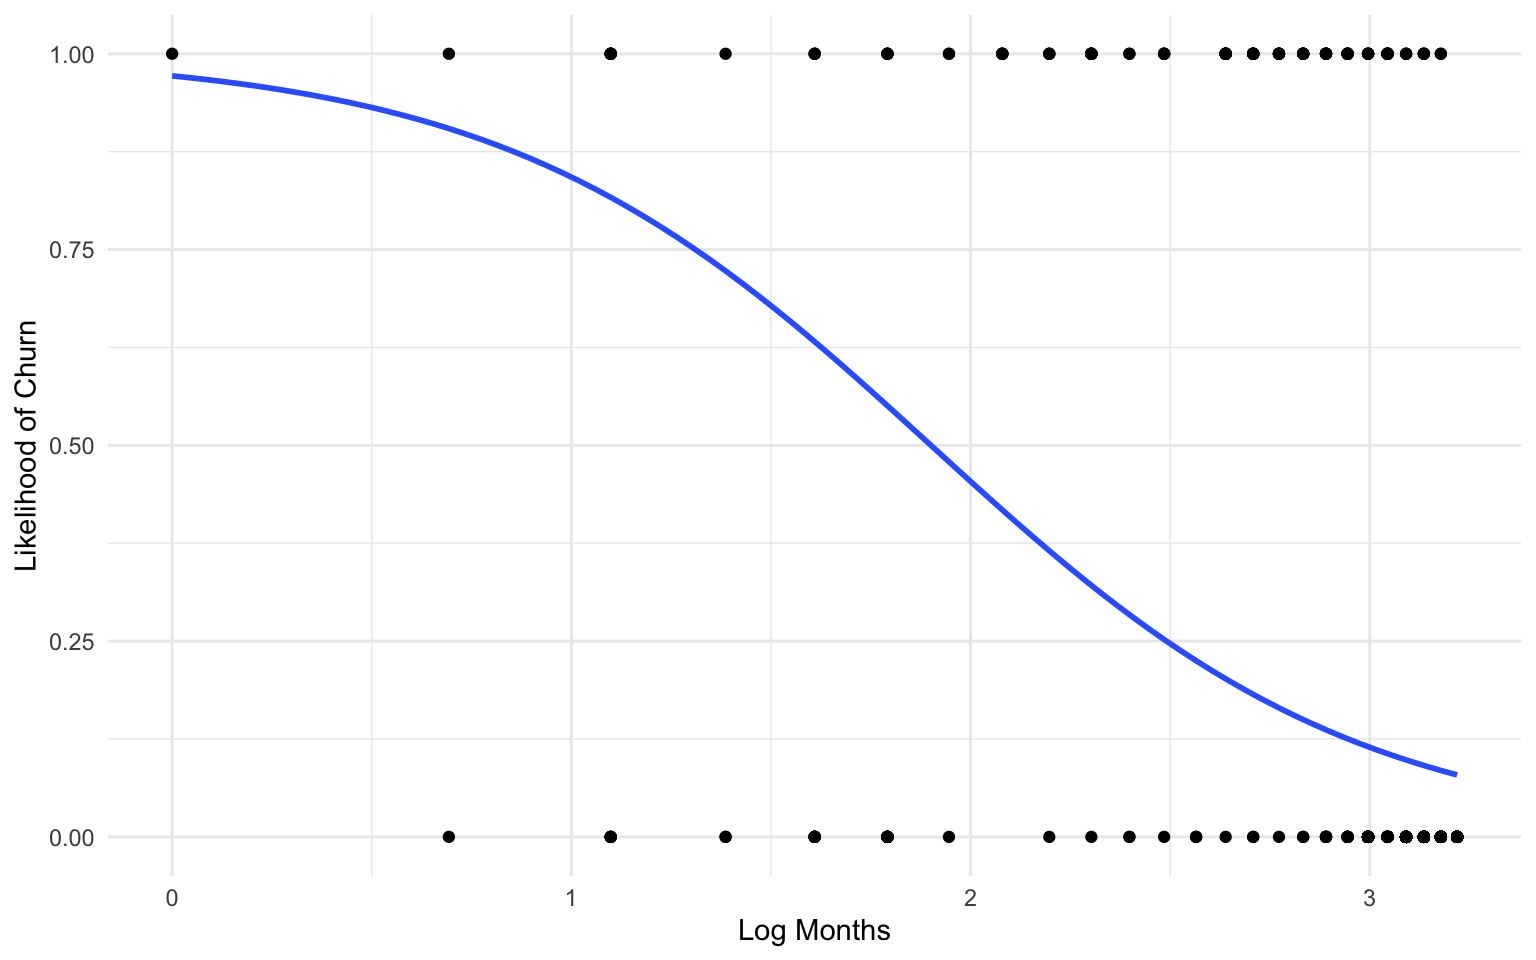
\includegraphics{/Users/jacobford/Documents/GitHub/SETO_Data_Analysis/community_priorities_files/figure-latex/unnamed-chunk-11-1.pdf}

\hypertarget{homeownership}{%
\subsubsection{Homeownership}\label{homeownership}}

\includegraphics{/Users/jacobford/Documents/GitHub/SETO_Data_Analysis/community_priorities_files/figure-latex/unnamed-chunk-13-1.pdf}

\hypertarget{model}{%
\subsection{Model}\label{model}}

A number of independent variables will be used for both contract
attributes and demographic data. Interaction variables will be tested
for significant, along with a initial stepwise regression to determine
which variables to initially include. The below equation is a summary of
the full model used in this analysis. The dependent variable is a binary
variable for contract adoption, \(y_{signup}\), where 1 signifies the
contract was adopted and 0 signifies it was not.

\begin{equation}

y_{signup} = \beta_{0} + \beta_{1}x_{sr} +\beta_{2}x_{cly} +\beta_{3}x_{clp}  +\beta_{4}x_{cf} + \\  \beta{5}x_{inc}+\beta_{6}x_{race} + \beta_{7}x_{hs} +\beta_{8}x_{fam} + \beta_{9}x_{rev} + \beta_{10}x_{ord}+ e_{i}

\end{equation}

where,

\begin{itemize}
\tightlist
\item
  \(x_{sr}\): savings rates on monthly energy bill in contracts, listed
  at either 5\%, 10\% or 20\%
\item
  \(x_{cly}\): contract length years, either 1 or 25 years
\item
  \(x_{clp}\): contract length pages, either 10 or 20 pages
\item
  \(x_{cf}\): cancellation fee, either zero or \$250
\item
  \(x_{inc}\): income, listed as Low (up to 50\% of AMI), Moderate (50\%
  - 120\% of AMI), or High (\textgreater120\% AMI)
\item
  \(x_{race}\): Categories include Asian, Black or African American,
  Hispanic or Latino, White and Other POC
\item
  \(x_{hs}\): Homeowner status for Homeowner, Renter or Other
\item
  \(x_{fam}\): More or less familiar with community solar
\item
  \(x_{rev}\): How much respondent reviewed the contract; up to half the
  contract review is captured by ``less review'', over half and up to
  the whole contract is ``more review''
\item
  \(x_{ord}\): Contract review order, likely not necessary.
\end{itemize}

Other variables of interest to consider: government program - x\_govt

\hypertarget{results}{%
\section{Results}\label{results}}

\hypertarget{primary-analysis}{%
\subsection{Primary Analysis}\label{primary-analysis}}

\hypertarget{regression-tables}{%
\subsection{Regression Tables}\label{regression-tables}}

\hypertarget{table-1}{%
\subsubsection{Table 1}\label{table-1}}

\begin{verbatim}
## 
## Regression Table 1
## ===========================================================================================
##                                                 Dependent variable:                        
##                          ------------------------------------------------------------------
##                                                       Sign Up                              
##                               (1)             (2)              (3)              (4)        
## -------------------------------------------------------------------------------------------
## Savings Rate 10%             0.125           0.126            0.126            0.127       
##                             (0.090)         (0.090)          (0.090)          (0.091)      
##                                                                                            
## Savings Rate 20%             0.089           0.090            0.090            0.082       
##                             (0.087)         (0.087)          (0.087)          (0.087)      
##                                                                                            
## Contract Length 25 Years                   -0.202***        -0.202***        -0.213***     
##                                             (0.076)          (0.076)          (0.076)      
##                                                                                            
## Contract Length 20 Pages                     -0.046          -0.046            -0.053      
##                                             (0.072)          (0.072)          (0.073)      
##                                                                                            
## Cancellation Fee 250                                          0.001            0.008       
##                                                              (0.075)          (0.075)      
##                                                                                            
## High Income                                                                    0.210       
##                                                                               (0.137)      
##                                                                                            
## Moderate Income                                                               0.561***     
##                                                                               (0.120)      
##                                                                                            
## Constant                    0.304***        0.426***        0.425***           0.118       
##                             (0.073)         (0.091)          (0.097)          (0.126)      
##                                                                                            
## -------------------------------------------------------------------------------------------
## Observations                 2,975           2,975            2,975            2,975       
## R2                           0.001           0.004            0.004            0.023       
## chi2                     1.964 (df = 2) 9.619** (df = 4) 9.619* (df = 5) 51.020*** (df = 7)
## ===========================================================================================
## Note:                                                           *p<0.1; **p<0.05; ***p<0.01
\end{verbatim}

\hypertarget{table-2}{%
\subsubsection{Table 2}\label{table-2}}

\begin{verbatim}
## 
## Regression Table 2
## ==========================================================================================================
##                                                         Dependent variable:                               
##                          ---------------------------------------------------------------------------------
##                                                               Sign Up                                     
##                                  (1)                 (2)                 (3)                  (4)         
## ----------------------------------------------------------------------------------------------------------
## Savings Rate 10%                0.115               0.120               0.158*               0.159*       
##                                (0.091)             (0.091)             (0.096)              (0.096)       
##                                                                                                           
## Savings Rate 20%                0.077               0.078               0.117                0.120        
##                                (0.088)             (0.088)             (0.094)              (0.094)       
##                                                                                                           
## Contract Length 25 Years      -0.209***           -0.223***           -0.229***            -0.226***      
##                                (0.076)             (0.077)             (0.081)              (0.081)       
##                                                                                                           
## Contract Length 20 Pages       -0.065              -0.065               -0.067               -0.057       
##                                (0.073)             (0.073)             (0.076)              (0.076)       
##                                                                                                           
## Cancellation Fee 250            0.013               0.012               0.037                0.041        
##                                (0.075)             (0.076)             (0.081)              (0.081)       
##                                                                                                           
## High Income                    0.290**              0.231              0.356**              0.348**       
##                                (0.144)             (0.146)             (0.157)              (0.158)       
##                                                                                                           
## Moderate Income               0.601***            0.540***             0.535***             0.526***      
##                                (0.122)             (0.124)             (0.132)              (0.132)       
##                                                                                                           
## Black                           0.075               0.162               0.089                0.073        
##                                (0.146)             (0.148)             (0.156)              (0.157)       
##                                                                                                           
## Hispanic                        0.224              0.319**              0.169                0.160        
##                                (0.153)             (0.158)             (0.169)              (0.170)       
##                                                                                                           
## Asian                          -0.136              -0.072               -0.017               0.004        
##                                (0.151)             (0.154)             (0.164)              (0.164)       
##                                                                                                           
## Other                          0.303*              0.376**             0.440**              0.442**       
##                                (0.177)             (0.179)             (0.189)              (0.190)       
##                                                                                                           
## Renter                                            -0.327***             -0.092               -0.070       
##                                                    (0.108)             (0.116)              (0.116)       
##                                                                                                           
## More Familiar                                                          1.470***             1.478***      
##                                                                        (0.110)              (0.110)       
##                                                                                                           
## More Reviewed                                                                               0.256**       
##                                                                                             (0.101)       
##                                                                                                           
## Constant                        0.026               0.167             -0.738***            -0.905***      
##                                (0.149)             (0.157)             (0.179)              (0.189)       
##                                                                                                           
## ----------------------------------------------------------------------------------------------------------
## Observations                    2,975               2,975               2,975                2,975        
## R2                              0.028               0.035               0.178                0.182        
## chi2                     62.852*** (df = 11) 79.180*** (df = 12) 421.368*** (df = 13) 430.983*** (df = 14)
## ==========================================================================================================
## Note:                                                                          *p<0.1; **p<0.05; ***p<0.01
\end{verbatim}

\hypertarget{odds-ratios}{%
\subsection{Odds Ratios}\label{odds-ratios}}

\hypertarget{table-1-1}{%
\subsubsection{Table 1}\label{table-1-1}}

\begin{verbatim}
## 
## Odds Ratio, Table 1
## ===========================================================================================
##                                                 Dependent variable:                        
##                          ------------------------------------------------------------------
##                                                       Sign Up                              
##                               (1)             (2)              (3)              (4)        
## -------------------------------------------------------------------------------------------
## Savings Rate 10%             1.133           1.134            1.134            1.136       
##                             (1.094)         (1.094)          (1.094)          (1.095)      
##                                                                                            
## Savings Rate 20%             1.093           1.095            1.095            1.085       
##                             (1.091)         (1.091)          (1.091)          (1.091)      
##                                                                                            
## Contract Length 25 Years                     0.817            0.817            0.808       
##                                             (1.079)          (1.079)          (1.079)      
##                                                                                            
## Contract Length 20 Pages                     0.955            0.955            0.949       
##                                             (1.075)          (1.075)          (1.076)      
##                                                                                            
## Cancellation Fee 250                                          1.001            1.008       
##                                                              (1.078)          (1.078)      
##                                                                                            
## High Income                                                                    1.234       
##                                                                               (1.147)      
##                                                                                            
## Moderate Income                                                                1.752       
##                                                                               (1.127)      
##                                                                                            
## Constant                     1.355           1.531            1.530            1.126       
##                             (1.076)         (1.096)          (1.101)          (1.134)      
##                                                                                            
## -------------------------------------------------------------------------------------------
## Observations                 2,975           2,975            2,975            2,975       
## R2                           0.001           0.004            0.004            0.023       
## chi2                     1.964 (df = 2) 9.619** (df = 4) 9.619* (df = 5) 51.020*** (df = 7)
## ===========================================================================================
## Note:                                                           *p<0.1; **p<0.05; ***p<0.01
\end{verbatim}

\hypertarget{table-2-1}{%
\subsubsection{Table 2}\label{table-2-1}}

\begin{verbatim}
## 
## Odds Ratio, Table 2
## ==========================================================================================================
##                                                         Dependent variable:                               
##                          ---------------------------------------------------------------------------------
##                                                               Sign Up                                     
##                                  (1)                 (2)                 (3)                  (4)         
## ----------------------------------------------------------------------------------------------------------
## Savings Rate 10%                1.121               1.128               1.172                1.172        
##                                (1.095)             (1.096)             (1.101)              (1.101)       
##                                                                                                           
## Savings Rate 20%                1.080               1.081               1.124                1.127        
##                                (1.092)             (1.092)             (1.098)              (1.098)       
##                                                                                                           
## Contract Length 25 Years        0.812               0.800               0.795                0.798        
##                                (1.079)             (1.080)             (1.085)              (1.085)       
##                                                                                                           
## Contract Length 20 Pages        0.937               0.937               0.935                0.944        
##                                (1.076)             (1.076)             (1.079)              (1.079)       
##                                                                                                           
## Cancellation Fee 250            1.014               1.012               1.038                1.042        
##                                (1.078)             (1.078)             (1.084)              (1.084)       
##                                                                                                           
## High Income                     1.336               1.260               1.427                1.416        
##                                (1.155)             (1.157)             (1.170)              (1.171)       
##                                                                                                           
## Moderate Income                 1.825               1.716               1.708                1.692        
##                                (1.129)             (1.132)             (1.141)              (1.141)       
##                                                                                                           
## Black                           1.078               1.176               1.094                1.076        
##                                (1.157)             (1.159)             (1.169)              (1.170)       
##                                                                                                           
## Hispanic                        1.251               1.376               1.184                1.173        
##                                (1.166)             (1.171)             (1.184)              (1.185)       
##                                                                                                           
## Asian                           0.873               0.931               0.983                1.004        
##                                (1.163)             (1.166)             (1.179)              (1.179)       
##                                                                                                           
## Other                           1.354               1.456               1.553                1.556        
##                                (1.193)             (1.196)             (1.209)              (1.209)       
##                                                                                                           
## Renter                                              0.721               0.912                0.932        
##                                                    (1.114)             (1.123)              (1.123)       
##                                                                                                           
## More Familiar                                                          4.349***             4.382***      
##                                                                        (1.116)              (1.116)       
##                                                                                                           
## More Reviewed                                                                                1.292        
##                                                                                             (1.106)       
##                                                                                                           
## Constant                        1.026               1.182               0.478                0.404        
##                                (1.160)             (1.170)             (1.196)              (1.208)       
##                                                                                                           
## ----------------------------------------------------------------------------------------------------------
## Observations                    2,975               2,975               2,975                2,975        
## R2                              0.028               0.035               0.178                0.182        
## chi2                     62.852*** (df = 11) 79.180*** (df = 12) 421.368*** (df = 13) 430.983*** (df = 14)
## ==========================================================================================================
## Note:                                                                          *p<0.1; **p<0.05; ***p<0.01
\end{verbatim}

\begin{enumerate}
\def\labelenumi{\arabic{enumi}.}
\tightlist
\item
  Table 1
\end{enumerate}

\begin{itemize}
\tightlist
\item
  Contract length of 25 years compared to 1 year remained a significant
  deterrent to contract acceptance rates.
\item
  Relative to low income, moderate and higher income respondents were
  more likely to accept the contract, holding th effect of savings rate,
  cancellation fee, and contract length constant.
\end{itemize}

\begin{enumerate}
\def\labelenumi{\arabic{enumi}.}
\setcounter{enumi}{1}
\tightlist
\item
  Table 2
\end{enumerate}

\begin{itemize}
\tightlist
\item
  Contract lenght remained a constant deterrance
\item
  Homeowner status, rent vs homeowner, was not observed as a
  statistically significant effect on signup rate. Likely some
  multicollinearity due to effect (sign) varying from model 2 to model
  4.
\item
  After including familiarity and reviewed dummies, savings rate becomes
  statistically significant effect on likelihood of contract adoption.
\item
  More familiar with community solar implies significantly more likely
  to adopt contract (suggests importance of education) - odds ratio of
  \textgreater4 in model 3 and 4
\item
  In looking at contract adoption by race, Hispanics were the only group
  observed with a statistically significant effect in models 1 and 2.
  Relative to white, hispanic rates were higher. This effect is negated
  after additional IVs are introduces in models 3 and 4.
\end{itemize}

From Table 1, four models are presented analyzing changes in probability
of sign up. Controlling for all other variables, contract length and
income were found to have statistically significant effects on the rate
of sign up. Contract length was found to have a strong negative impact
on probability of contract adoption. For example, holding all variables
constant, from model 2 we see that the odds ratio for contract length of
25 years is 0.782, meaning the group with contracts of 25 years are
0.782 times as likely as the group with contracts of 1 year of signing
up, or a 21.8\% decrease in odds of signing up.

Interestingly, lower income respondents were much less likely to adopt
the contract, even when controlling for savings rate, contract length
and number of pages, and cancellation fees. High income and medium
income respondents were 1.3 and 1.7 times the odds to adopt the contract
compared to low income respondents, controlling for contract attributes.

\hypertarget{secondary-analysis}{%
\subsection{Secondary Analysis}\label{secondary-analysis}}

The secondary analysis will include an ordered logit model to
investigate the degree of which the same independent variables above
influence the likert scale questions asked in the survey. Ordered logit
models are commonly utilized with outputs of interest are categorized in
discrete sequences, such as a Likert scale.

\hypertarget{wouldwould-not-sign-up}{%
\subsection{Would/Would Not Sign Up}\label{wouldwould-not-sign-up}}

\hypertarget{savings-rate}{%
\subsubsection{Savings Rate}\label{savings-rate}}

Tables 1-4 in output/regressions

\hypertarget{agreedisagree}{%
\subsection{Agree/Disagree}\label{agreedisagree}}

\hypertarget{discussion}{%
\section{Discussion}\label{discussion}}

\end{document}
